% Editable master. Rebuild the PDF and theme-aware SVG with: python3 build.py
% The curves are the bound q^k E_0 with E_0 = 1, not simulated iterations.
% Each marker is the smallest k with q^k E_0 <= epsilon_e = 1e-3:
% ceil(ln(1000)/(-ln q)) = 10, 31, and 66 for q = 0.5, 0.8, and 0.9.
\documentclass[10pt,border=10pt]{standalone}
\usepackage[T1]{fontenc}
\usepackage{helvet}
\usepackage{amsmath,amssymb}
\renewcommand{\familydefault}{\sfdefault}
\usepackage{pgfplots}
\pgfplotsset{compat=1.18}
\definecolor{ink}{HTML}{1E293B}
\definecolor{muted}{HTML}{536277}
\definecolor{fast}{HTML}{2463A8}
\definecolor{middle}{HTML}{137B69}
\definecolor{slow}{HTML}{E08A14}
\begin{document}
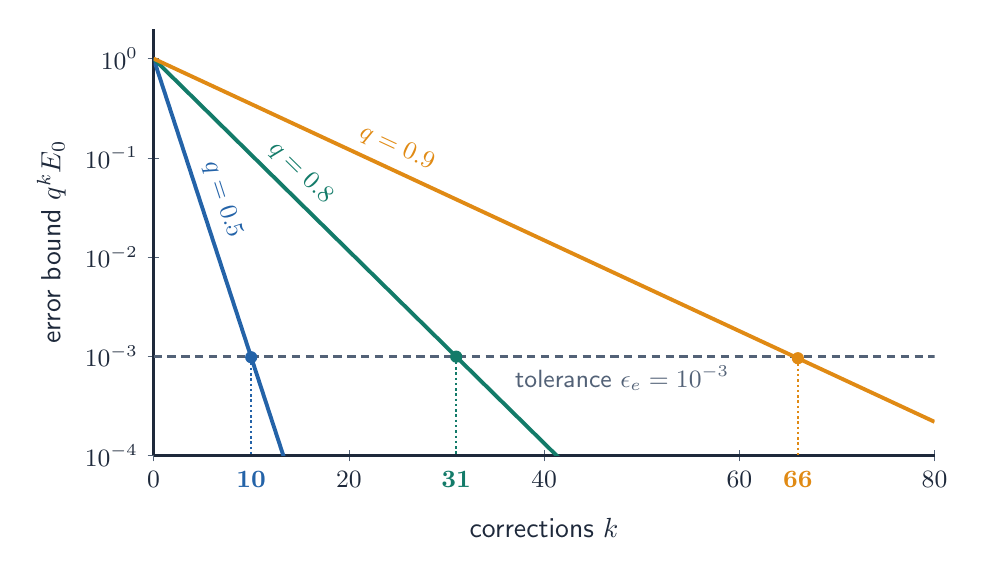
\begin{tikzpicture}
\begin{axis}[
  width=11.5cm, height=7cm,
  ymode=log, xmin=0, xmax=80, ymin=1e-4, ymax=2,
  axis lines=left, axis line style={draw=ink, line width=.8pt, -},
  tick style={draw=muted}, yminorticks=false,
  xtick={0,20,40,60,80}, ytick={1,1e-1,1e-2,1e-3,1e-4},
  extra x ticks={10,31,66},
  extra x tick labels={$\textcolor{fast}{\mathbf{10}}$,
    $\textcolor{middle}{\mathbf{31}}$, $\textcolor{slow}{\mathbf{66}}$},
  extra x tick style={tick style={draw=none}},
  ticklabel style={font=\sffamily\small, text=ink},
  xlabel={corrections $k$}, ylabel={error bound $q^{k}E_0$},
  label style={font=\sffamily, text=ink},
  every axis plot/.append style={line width=1.4pt},
]
  % Tolerance on the solution error.
  \addplot[muted, densely dashed, line width=1pt, domain=0:80, samples=2] {1e-3};
  \node[font=\sffamily\small, text=muted, anchor=north] at (axis cs:48,1e-3)
    {tolerance $\epsilon_e=10^{-3}$};

  % Error bounds. Axis clipping trims each line at the bottom of the plot.
  \addplot[fast, domain=0:15, samples=40] {0.5^x}
    node[pos=.33, above, sloped, font=\sffamily\small, text=fast] {$q=0.5$};
  \addplot[middle, domain=0:45, samples=60] {0.8^x}
    node[pos=.30, above, sloped, font=\sffamily\small, text=middle] {$q=0.8$};
  \addplot[slow, domain=0:80, samples=80] {0.9^x}
    node[pos=.30, above, sloped, font=\sffamily\small, text=slow] {$q=0.9$};

  % First correction count that meets the tolerance.
  \draw[fast, densely dotted, line width=.9pt] (axis cs:10,{0.5^10}) -- (axis cs:10,1e-4);
  \draw[middle, densely dotted, line width=.9pt] (axis cs:31,{0.8^31}) -- (axis cs:31,1e-4);
  \draw[slow, densely dotted, line width=.9pt] (axis cs:66,{0.9^66}) -- (axis cs:66,1e-4);
  \fill[fast] (axis cs:10,{0.5^10}) circle (2.2pt);
  \fill[middle] (axis cs:31,{0.8^31}) circle (2.2pt);
  \fill[slow] (axis cs:66,{0.9^66}) circle (2.2pt);
\end{axis}
\end{tikzpicture}
\end{document}
